% !TEX TS-program = pdflatex
% !TEX encoding = UTF-8 Unicode

% This is a simple template for a LaTeX document using the "article" class.
% See "book", "report", "letter" for other types of document.

\documentclass[11pt]{article} % use larger type; default would be 10pt

\usepackage[utf8]{inputenc} % set input encoding (not needed with XeLaTeX)

%%% Examples of Article customizations
% These packages are optional, depending whether you want the features they provide.
% See the LaTeX Companion or other references for full information.

%%% PAGE DIMENSIONS
\usepackage{geometry} % to change the page dimensions
\geometry{letterpaper} % or letterpaper (US) or a5paper or....
% \geometry{margins=2in} % for example, change the margins to 2 inches all round
% \geometry{landscape} % set up the page for landscape
%   read geometry.pdf for detailed page layout information

\usepackage{graphicx} % support the \includegraphics command and options

% \usepackage[parfill]{parskip} % Activate to begin paragraphs with an empty line rather than an indent

%%% PACKAGES
\usepackage{booktabs} % for much better looking tables
\usepackage{array} % for better arrays (eg matrices) in maths
\usepackage{paralist} % very flexible & customisable lists (eg. enumerate/itemize, etc.)
\usepackage{verbatim} % adds environment for commenting out blocks of text & for better verbatim
\usepackage{subfig} % make it possible to include more than one captioned figure/table in a single float
\usepackage{amsmath}
\usepackage{amssymb}
\usepackage{listings}
% These packages are all incorporated in the memoir class to one degree or another...

%%% HEADERS & FOOTERS
\usepackage{fancyhdr} % This should be set AFTER setting up the page geometry
\pagestyle{fancy} % options: empty , plain , fancy
\renewcommand{\headrulewidth}{0pt} % customise the layout...
\lhead{}\chead{}\rhead{}
\lfoot{}\cfoot{\thepage}\rfoot{}

%%% SECTION TITLE APPEARANCE
\usepackage{sectsty}
\allsectionsfont{\sffamily\mdseries\upshape} % (See the fntguide.pdf for font help)
% (This matches ConTeXt defaults)

%%% ToC (table of contents) APPEARANCE
\usepackage[nottoc,notlof,notlot]{tocbibind} % Put the bibliography in the ToC
\usepackage[titles,subfigure]{tocloft} % Alter the style of the Table of Contents
\renewcommand{\cftsecfont}{\rmfamily\mdseries\upshape}
\renewcommand{\cftsecpagefont}{\rmfamily\mdseries\upshape} % No bold!

%%% END Article customizations

%%% The "real" document content comes below...

\title{CS267 Assignment 3}
\author{Patrick Li, Simon Scott}
%\date{} % Activate to display a given date or no date (if empty),
         % otherwise the current date is printed 

\begin{document}
\maketitle
\parskip 7.2pt

\section{Aims}
The aim of this assignment was to 
\begin{enumerate}
  \item find and fix the race condition in the supplied implementation of knapsack using Thrille, and
  \item develop a correct parallel implementation of dynamic programming to solve the 0-1 knapsack problem that demonstrates weak and strong scaling.
\end{enumerate}

\section{Debugging using Thrille}
\subsection{Detected Race Condition}
{\tiny
\begin{lstlisting}
UPCR: UPC thread 0 of 4 on nid12594 (process 0 of 4, pid=27595)
UPCR: UPC thread 3 of 4 on nid12597 (process 3 of 4, pid=27135)
UPCR: UPC thread 2 of 4 on nid12596 (process 2 of 4, pid=27623)
UPCR: UPC thread 1 of 4 on nid12595 (process 1 of 4, pid=27581)
Initializing Race Detection 0.9.18 (BACK_OFF=0.95, EPS=4.65661e-10)...
[0] Potential race #1 found:
[0] Read from [0x3df4000,0x3df4004) by thread 1 at phase 0 
    (knapsack-race.upc:34:upcr_addrfield_pshared(v)+(0)@0x5127a0)
[0] Write to [0x3df4000,0x3df4004) by thread 0 at phase 0 
    (knapsack-race.upc:143:upcr_addrfield_pshared(_bupc_Mptra67)+(0)@0x512f80)
[0] Potential race #2 found:
[0] Read from [0x3df6000,0x3df6004) by thread 1 at phase 0 
    (knapsack-race.upc:33:upcr_addrfield_pshared(w)+(0)@0x512768)
[0] Write to [0x3df6000,0x3df6004) by thread 0 at phase 0 
    (knapsack-race.upc:142:upcr_addrfield_pshared(_bupc_Mptra66)+(0)@0x512f40)
[2] Local shared reads: 0 / writes: 0
<>[1] Local shared reads: 0 / writes: 0
<>[3] Local shared reads: 0 / writes: 0
<>5000 items, capacity: 999, time: 8.79658
82 items used, value 53454, weight 999
Exiting Race Detection 0.9.18...
[0] Local shared reads: 0 / writes: 0
\end{lstlisting}
}

\subsection*{knapsack-race.upc:143}
{\tiny
\begin{lstlisting}
max_weight = min( max_weight, capacity );
upc_forall( i = 0; i < nitems; i++; i )
{
   weight[i] = 1 + (lrand48()%max_weight); <- WRITE
   value[i]  = 1 + (lrand48()%max_value);  <- WRITE
}
\end{lstlisting}
}

\subsection*{knapsack-race.upc:33 in build\_table}
{\tiny
\begin{lstlisting}
wj = w[0]; <- READ
vj = v[0]; <- READ
upc_forall( int i = 0;  i <  wj;  i++; &T[i] ) T[i] = 0;
upc_forall( int i = wj; i <= cap; i++; &T[i] ) T[i] = vj;
\end{lstlisting}
}

\subsection{Explanation of Race Condition}

In build\_table, each thread incrementally reads from the weight and value array, starting from the first element, in order to build the T table, one row at a time. However, this assumes, incorrectly, that the weight and value array has been properly initialized. weight[0] and value[0] is initialized by thread 0 (MYTHREAD == 0). Incorrect behavior results from thread 1 reads from weight[0] and value[0] before they are initialized by thread 0.

\subsection{Fix for Race Condition}
We can prevent the race condition by using a upc\_barrier statement to ensure that the weight and value array is initialized before calling build\_table. 

{\tiny
\begin{lstlisting}
max_weight = min( max_weight, capacity );
upc_forall( i = 0; i < nitems; i++; i )
{
   weight[i] = 1 + (lrand48()%max_weight);
   value[i]  = 1 + (lrand48()%max_value);
}
upc_barrier; //Wait for initialization to complete
\end{lstlisting}
}

\subsection{No More Detected Races}
Running Thrille on the fixed source results in no more detected race conditions.

{\tiny
\begin{lstlisting}
UPCR: UPC thread 0 of 4 on nid02346 (process 0 of 4, pid=11575)
UPCR: UPC thread 3 of 4 on nid02349 (process 3 of 4, pid=11584)
UPCR: UPC thread 2 of 4 on nid02348 (process 2 of 4, pid=11581)
UPCR: UPC thread 1 of 4 on nid02347 (process 1 of 4, pid=11578)
Initializing Race Detection 0.9.18 (BACK_OFF=0.95, EPS=4.65661e-10)...
[2] Local shared reads: 0 / writes: 0
<>[3] Local shared reads: 0 / writes: 0
<>[1] Local shared reads: 0 / writes: 0
<>5000 items, capacity: 999, time: 8.58934
75 items used, value 52721, weight 997
Exiting Race Detection 0.9.18...
[0] Local shared reads: 0 / writes: 0
\end{lstlisting}
}

\section{Method of Parallelization}

The dynamic programming matrix, \emph{T}, has NITEMS rows and CAPACITY columns. This matrix is computed in parallel by allocating NITEMS/\emph{P} adjacent columns, to each processor, where \emph{P} is the number of processors. Therefore, non-cyclic column blocking is used to partition the array.

Since each element in the table is dependent on two values in the row immediately above it, the threads are synchronized after computing each row.

\section{Optimization Techniques}

\subsection{Only Store Two Rows}
A straightforward implementation of dynamic programming to solve the 0-1 knapsack problem constructs and populates a NITEMS $\times$ CAPACITY table, $T$. After populating $T$, the optimal value is found at $T[\text{NITEMS}, \text{CAPACITY}]$. To find the subset of items contained in the knapsack we backtrack along the rows of the table and determine whether each item was included in the knapsack. 

We are interested only in the total weight, value, and the final number of items in the table, and \emph{not} the actual subset of items that were used. Hence, we can save memory by not storing the entire $T$ table. At any time we only need to store 2 rows of the table, the current row that we are calculating, and the previous row, on which the current row depends on.

\subsection{Elimination of Backtracking}

Backtracking along each row of $T$ to determine the final number of items in the knapsack is expensive. Instead, we keep track of the number of items used for each weight in a separate 1$\times$C array, \emph{count}, and update \emph{count} during the calculation of $T$. For each item $i$, we may choose to either include it in the knapsack, at which time \emph{count}$_i$ is incremented, or we may choose to exclude it from knapsack, keeping \emph{count}$_i$ unmodified.

Because all items have a positive value, the total value in the knapsack changes with each additional item included. Therefore, the final weight in the knapsack can be computed by looking, in the last row of $T$, for the last column at which the total value changes. I.e. we look for the largest weight i, at which $T[\text{NITEMS}, i] > T[\text{NITEMS}, i-1]$.

With the above two modifications to the original implementation, we avoid the backtracking phase of the computation.

\subsection{Bulk Memory Copies}

To compute each element in the dynamic programming matrix, the algorithm must take the maximum of two values in the row above. The one element is directly above, while the other is above and to the left. In Figure~\ref{memcpy_diagram}, the yellow element in \emph{Row i} is dependent on the two yellow elements in \emph{Row i-1}. Furthermore, adjacent elements in the current row (the blue items in the figure) are dependent on the elements directly above (the red elements) and an \emph{adjacent} set of elements to left (the green elements). The red elements are stored on the current processor, while the green elements are stored on 1 or 2 other processors.

\begin{figure}
\begin{centering}
\includegraphics*[width=0.5\paperwidth, viewport= 70 575 540 720]{figures/memcpy_diagram.pdf}
\caption{Dependencies between Elements in the Matrix}
\label{memcpy_diagram}
\end{centering}
\end{figure}

In a naive implementation, CPU 2 would read each green element one at a time to compute the blue items. This results in many network accesses and is therefore slow. Instead, the entire green block of data is copied into a local temporary buffer, using one or two UPC \emph{memget} operations. CPU 2 therefore accesses the network at most twice, instead of once for each element, making it much faster.

\subsection{Synchronizing via Spin-Locks}

Computing any row of $T$ requires the values from the previous row. The straightforward implementation uses a upc\_barrier statement to ensure that all threads have completed calculating the previous row before we begin calculating the current row. However, barriers incur significant overhead because they require the coordination of every running thread. By noticing that each individual element in $T$, $T[w,c]$, is dependent upon only a small number of other elements, $T[w,c-1]$ and $T[w-w_c,c-1]$, we can replace the course upc\_barrier statement with a finer synchronization primitive that only requires coordination between dependent threads. We let the computation for $T[w,c]$ proceed as soon as $T[w,c-1]$ and $T[w-w_c,c-1]$ are finished computing.

To keep track of the progress of each thread, we use a shared 1$\times$THREADS \emph{progress} array. Each element in \emph{progress} indicates the last row of $T$ that has finished computing. Thus before computing $T[w,c]$ we check whether \emph{progress}$[t] \geq c-1$, where $t$ is the thread responsible for computing $T[w-w_c,c-1]$, and otherwise wait using a spin-lock. To prevent the UPC compiler from optimizing away the spin-lock, \emph{progress} must be declared as \emph{volatile}.

\section{Results}

\subsection{Strong Scaling}

\begin{figure}
\begin{centering}
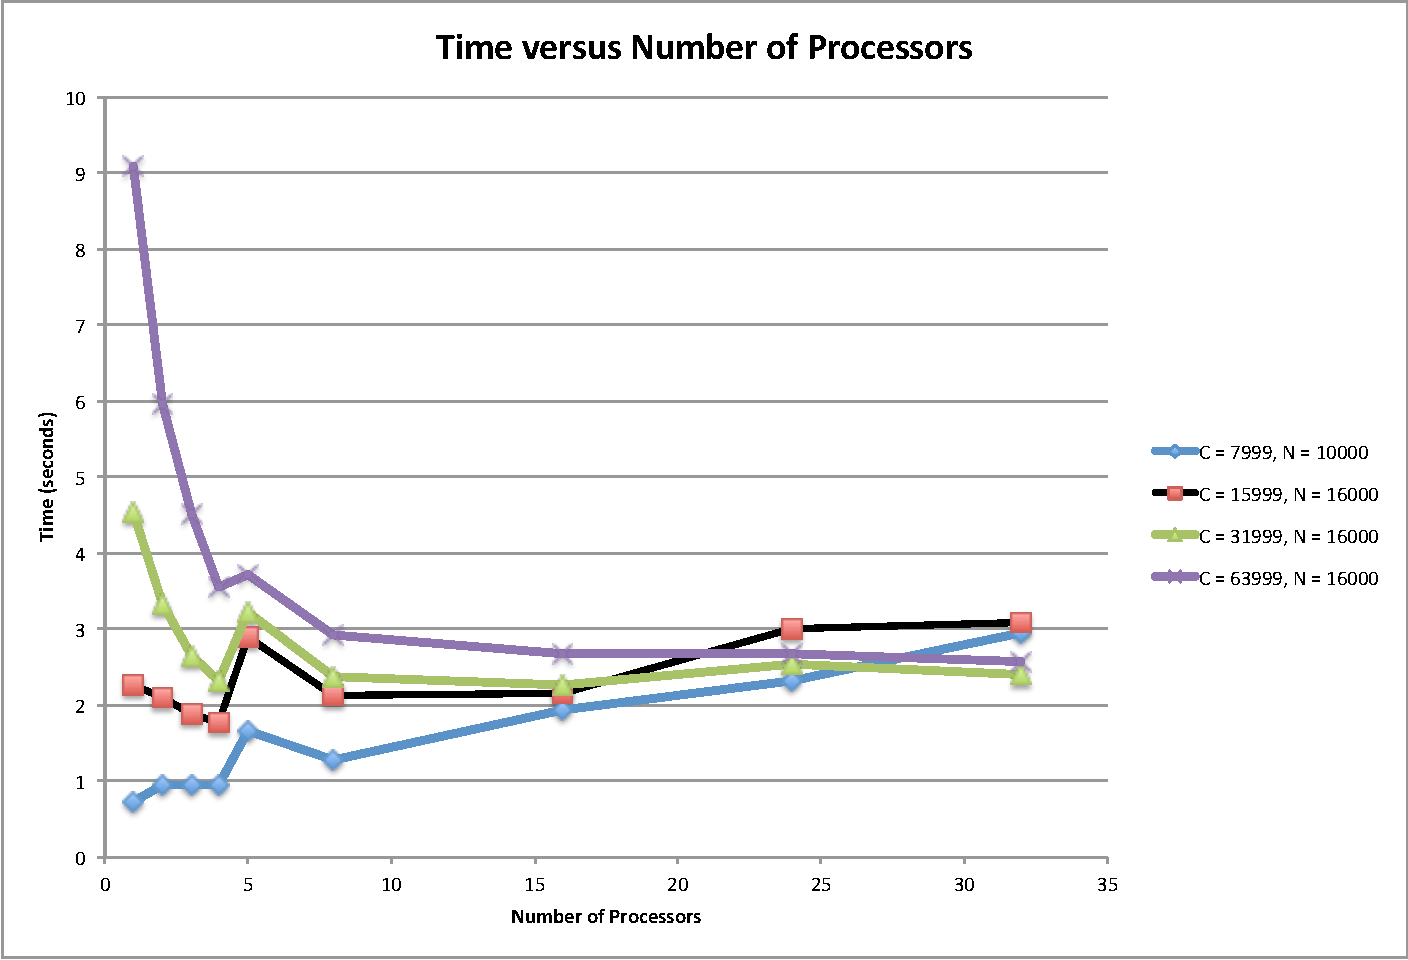
\includegraphics[width=0.5\paperwidth]{figures/TvsP.pdf}
\caption{Time versus Number of Processors}
\label{TvsP}
\end{centering}
\end{figure}

Figure \ref{TvsP} shows how the execution time scales with the number of processors for a number of different problem sizes. We see that there is significant communication overhead from running across multiple processors, as when problem sizes are too small ($C = 7999$) execution time actually \emph{increases} with the number of processors. As problem sizes increase, additional processors decrease execution time. In the case of $C = 63999$, we achieve a 64\% parallelization efficiency as the number of processors increase from 1 to 4. At $P = 5$, we see a sharp bump up in execution times due to the additional overhead of internode communication.

\subsection{Weak Scaling}

\begin{figure}
\begin{centering}
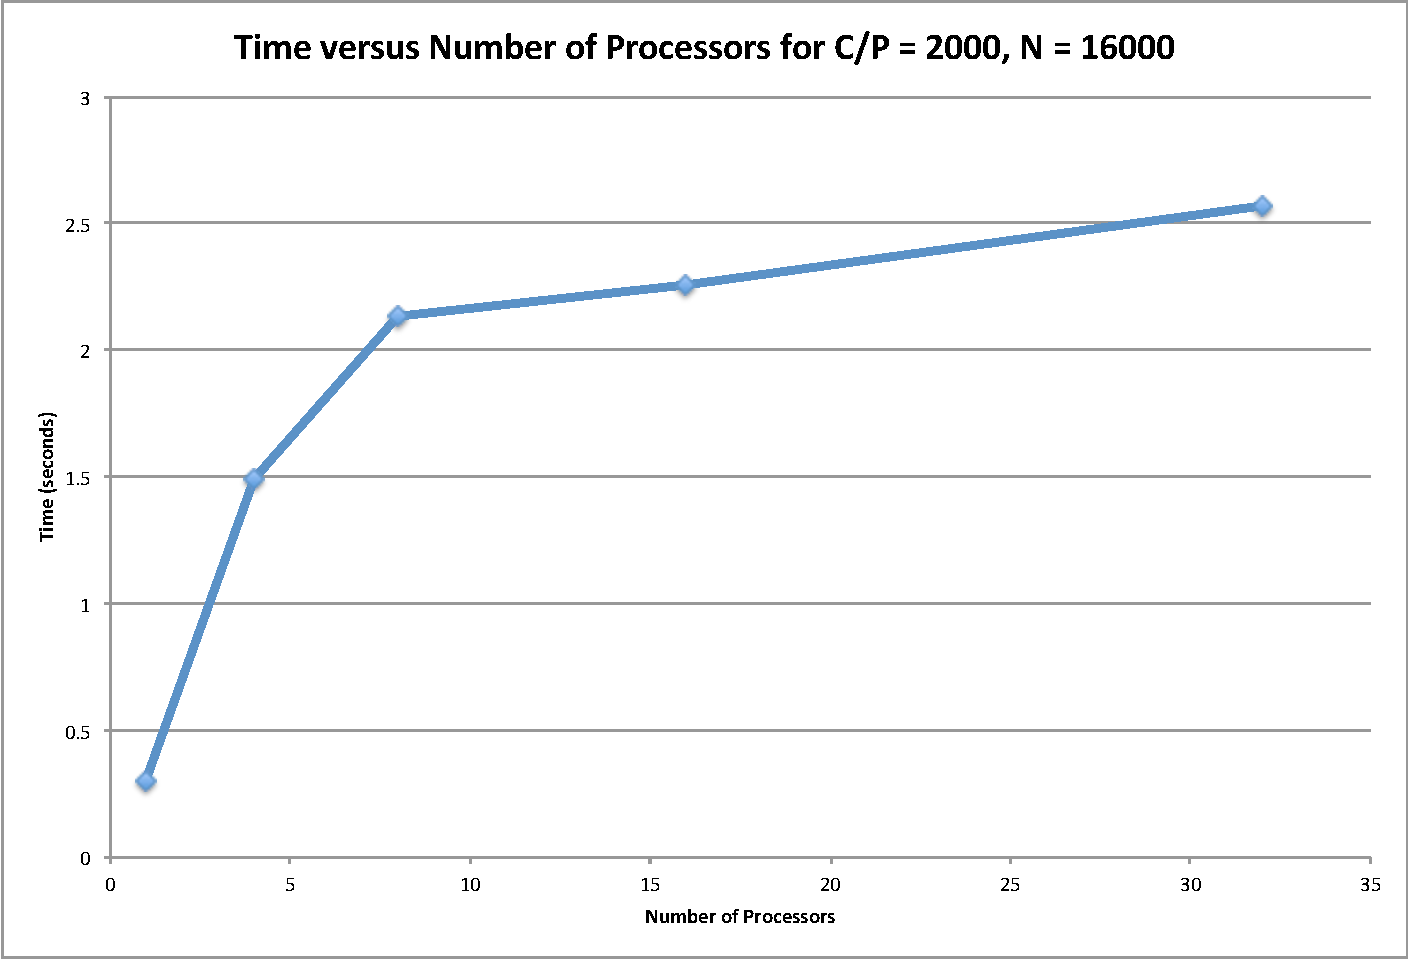
\includegraphics[width=0.5\paperwidth]{figures/TvsP-fixed.pdf}
\caption{Time versus Number of Processors for a Fixed C/P}
\label{TvsP-fixed}
\end{centering}
\end{figure}

Figure \ref{TvsP-fixed} shows how the execution time scales with the number of processors for a fixed problem size $C/P = 2000$. Under 100\$ parallelization efficiency, the curve should be flat, whereas in our case the curve starts with a relatively high slope and then flattens out as the number of processors increase. The increase in execution time from $P = 1$ to $P = 4$ is due to the additional overhead of intercore communication and synchronization. The increase in execution time from $P = 4$ to $P = 8$ is due to the additional overhead of internode communication and synchronization. After $P = 8$ the curve is nearly flat, with the remaining overhead due to the propagation of information from capacity $c = 0$ to $c = C$.

\subsection{Time versus Problem Size}

\begin{figure}
\begin{centering}
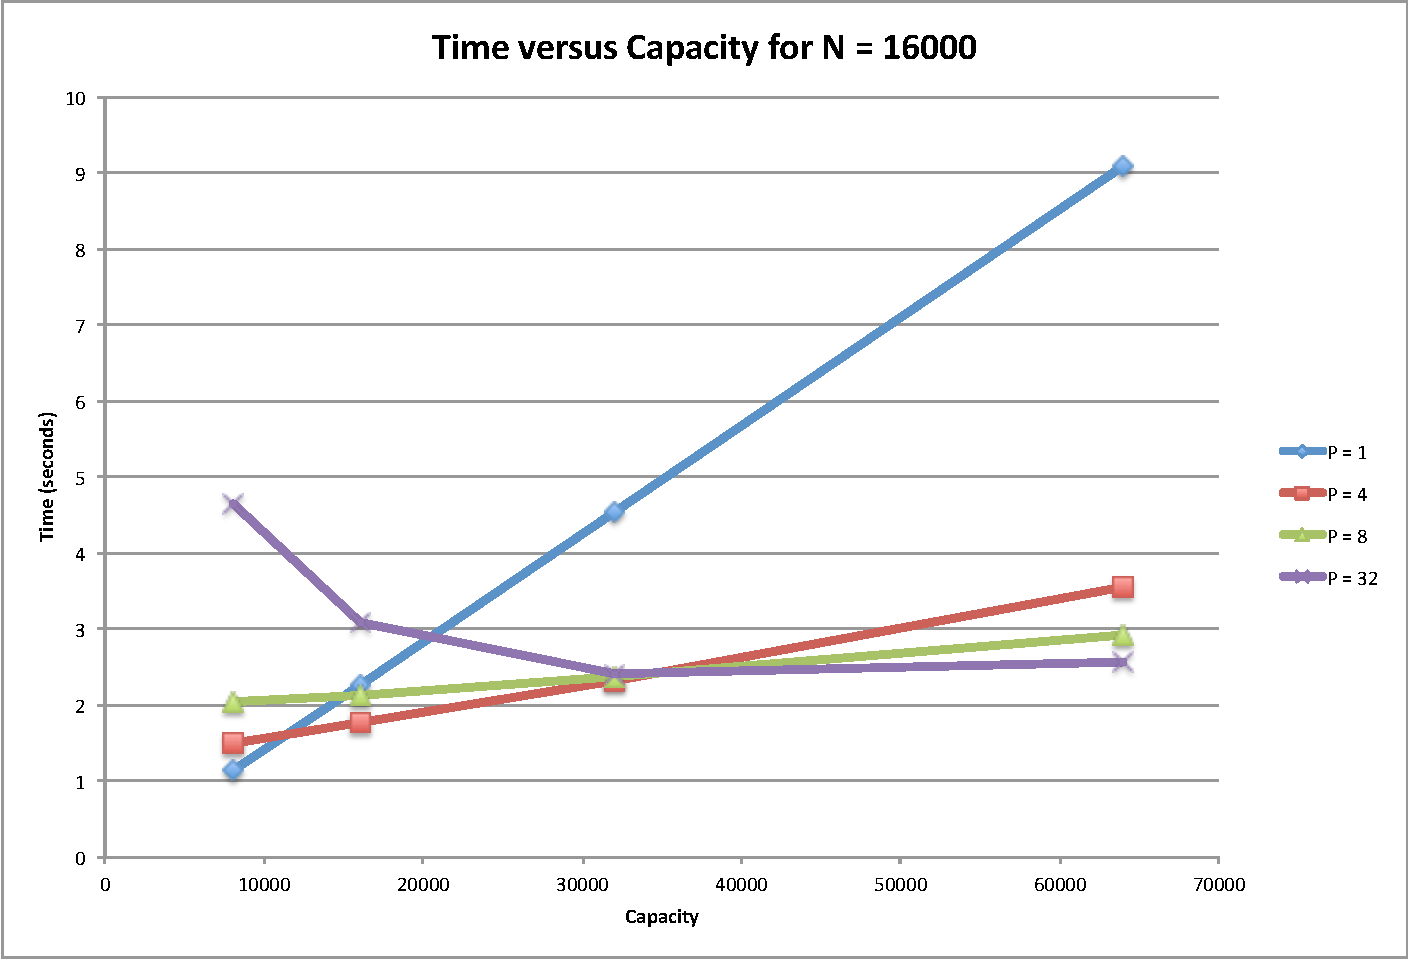
\includegraphics[width=0.5\paperwidth]{figures/TvsC.pdf}
\caption{Time versus Capacity for N = 16000}
\label{TvsC}
\end{centering}
\end{figure}

How does solution time vary for fixed number of processors, when problem sized increased. Shows figure 2, and explain.

\subsection{Effect of Optimizations on Performance}

\subsubsection{Bulk Memory Copies}

Give \% speed increase for a single P, C, N combination.

\subsubsection{Synchronizing via Spin-Locks}

Give \% speed increase for a single P, C, N combination.

\section{Conclusion}

TODO

\end{document}
